%praktikrapport
\documentclass[11pt,a4paper,danish]{article}
\usepackage[utf8]{inputenc}
\usepackage[danish]{babel} % danske overskrifter
\usepackage[T1]{fontenc} % fonte (output)
\usepackage{graphicx} % indsættelse af billeder
\usepackage{caption}
\usepackage{subcaption}
\usepackage{wrapfig}
\usepackage{geometry}
\usepackage{titlesec}
\usepackage{fancyhdr}
\usepackage{lastpage}
\usepackage{hyperref}
\usepackage{gensymb}

\usepackage{setspace}
\usepackage{tocloft}
\usepackage{parskip}

% \permil
\usepackage{wasysym}

\usepackage[nottoc]{tocbibind}

%\usepackage{subfig}
%\usepackage{inconsolata}
%\usepackage{enumitem}

\titleformat{\paragraph}[runin]
{\bfseries\scshape}{\theparagraph}{1em}{}

% BEGIN JAVA CODE SECTION
\usepackage{listings}
\usepackage{color}

\definecolor{dkgreen}{rgb}{0,0.6,0}
\definecolor{gray}{rgb}{0.5,0.5,0.5}
\definecolor{mauve}{rgb}{0.58,0,0.82}

\lstset{frame=none,
	language=Java,
	aboveskip=3mm,
	belowskip=3mm,
	showstringspaces=false,
	columns=flexible,
	basicstyle={\small\ttfamily},
	numbers=none,
	numberstyle=\tiny\color{gray},
	keywordstyle=\color{blue},
	commentstyle=\color{dkgreen},
	stringstyle=\color{mauve},
	breaklines=true,
	breakatwhitespace=true,
	tabsize=2
}
% END JAVA CODE SECTION

% BEGIN C++ code
\definecolor{listinggray}{gray}{0.9}
\definecolor{lbcolor}{rgb}{0.9,0.9,0.9}
\lstset{
	backgroundcolor=\color{lbcolor},
	tabsize=4,
	%   rulecolor=,
	language=[GNU]C++,
	basicstyle=\scriptsize,
	upquote=true,
	aboveskip={1.5\baselineskip},
	columns=fixed,
	showstringspaces=false,
	extendedchars=false,
	breaklines=true,
	prebreak = \raisebox{0ex}[0ex][0ex]{\ensuremath{\hookleftarrow}},
	frame=single,
	numbers=left,
	showtabs=false,
	showspaces=false,
	showstringspaces=false,
	identifierstyle=\ttfamily,
	keywordstyle=\color[rgb]{0,0,1},
	commentstyle=\color[rgb]{0.026,0.112,0.095},
	stringstyle=\color[rgb]{0.627,0.126,0.941},
	numberstyle=\color[rgb]{0.205, 0.142, 0.73},
	%        \lstdefinestyle{C++}{language=C++,style=numbers}’.
}
\lstset{
	backgroundcolor=\color{lbcolor},
	tabsize=4,
	language=C++,
	captionpos=b,
	tabsize=3,
	frame=lines,
	numbers=left,
	numberstyle=\tiny,
	numbersep=5pt,
	breaklines=true,
	showstringspaces=false,
	basicstyle=\footnotesize,
	%  identifierstyle=\color{magenta},
	keywordstyle=\color[rgb]{0,0,1},
	commentstyle=\color{Darkgreen},
	stringstyle=\color{red}
}
%END C++ code

%\setcounter{secnumdepth}{3}

\geometry{
	a4paper,
	total={210mm,297mm},
	left=20mm,
	right=20mm,
	top=40mm,
	bottom=20mm,
}

\pagestyle{fancy}
\fancyhf{}
\rhead{Delta, \date{\today}}
\lhead{Rudy Alex Kohn}
\chead{Afsluttende}
\cfoot{Side \thepage \hspace{1pt} af \pageref{LastPage}}

% TOC som links
\usepackage{hyperref}
\hypersetup{
	colorlinks,
	citecolor=black,
	filecolor=black,
	linkcolor=black,
	urlcolor=blue
}

\title{Stripetykkelsesmåler\\Praktikrapport}
\author{Rudy Alex Kohn}
\date{24. Juli 2017}

\setlength{\parindent}{0pt}

\begin{document}
	
	\maketitle
	\renewcommand{\contentsname}{Indeks}
	\renewcommand{\listfigurename}{Figurliste}
	\renewcommand{\figurename}{Figur}
	\renewcommand\refname{Referencer}
	%PWNED! :> nice!
	
	\begin{center}
		Rudy Alex Kohn\\
		ruak@force.dk\\
		s133235@student.dtu.dk
	\end{center}
	
	\vspace{25mm}
	
	\begin{center}
		
\includegraphics[scale=0.3]{Billeder/kunlogo.png}
		
\includegraphics[scale=0.15]{Billeder/DELTA_1024px.png}
	\end{center}
	
	\newpage
	\setlength\cftparskip{-2pt}
	%\setlength\cftbeforechapskip{0.0pt}\singlespacing
	\tableofcontents
	%\singlespacing
	
	\listoffigures
	\listoftables
	
	%1:  produktspecifikation. forudsætninger
	%Performance  tykkelsesmålinh præsisosn +/- 0.1 mm
	%Product cist max 25,000,- kr gerne mindre.
	%2 teknologier og teknologi valg – begrundelse
	%3 forsøgsopstilling – gennemgang.
	%4 databehandling  procesdiagram.
	%5 resulateter  - hvordan ser det ud.
	%6 Videre arbejde- plan for den sidste del af projektet- hvor langt når vi, dokumentation etc.

	%PraktikDelta
\section{DELTA}

\subsection{Lidt om}
DELTA Road Sensors er afdelingen hvor der udvikles produkter der er vejrelaterede. F.eks. skiltemåler, vejstribe RL målere både som håndholdt og mobil. Der eksisterer kunder verden over, og det er typisk instanser der tilsvarer det danske vejdirektorat der er kunder.

\subsection{Afdelingen}
Da både hardware- og sofwaredele bliver udviklet helt fra bunden, spiller softwareudviklerne en stor rolle i hele processen. Dette reflekteres i deres konstante involvering i processen samt at de typisk skal have et dybt kendskab til produktet. Grundet denne viden udøver de også support på produkterne, hvilket er en meget vigtig del af det samlede salg, da nogle af produkter ligger på omkring en million.

\subsection{Udviklingsmetoderne}
På afdelingen findes der ikke nogen forskrifter til hvorledes produkterne udvikles og hvilke værktøjer der skal bruges. De enkelte udviklere besidder fuld kontrol over hvorledes det skal foregå, hvilket giver en høj grad af fleksibilitet, men kræver at hver udvikler skal som udgangspunkt være kendt med alle de gængse metoder og sprog.

\subsection{Samarbejde med andre afdelinger}
Afdelingerne fungerer som enkelte instanser.
Det resulterer derfor i at de forskellige afdelinger tager betaling fra hinanden internt, for at holde styr på hvor meget tid der bliver brugt på hvad, og hvordan det ser ud økonomisk i forhold til budgettet. DELTA er meget bevidst omkring hvad de bruger deres budget, og sørger for at alt bliver dokumenteret og at de korrekte afdelinger "betaler" hvad de skal til hinanden af samme årsag.




	
	%PraktikOpgaven
\section{Praktikopgaven}
Opgaven er et afklaringsprojekt. Det går ud på hvorvidt det er muligt at kunne måle tykkelsen af en vejstribe, der typisk er af thermoplast med reflekterende elementer som f.eks. små perler.

\section{Bevæggrunden}
Virksomhederne der anlægger vejstriberne har interesse i at kunne være sikker på hvor meget de rent faktisk bruger, og at de opfylder de krav kunder har ønsket, og ikke har unødigt spild. Kunderne kan verificere den tykkelse der er ønsket, og over tid estimere stribernes levetid, da disse bliver slidt ved brug. En kunde kan derfor følge op over en længere periode hvorledes slitage påvirker striberne og hvornår det kan være nødvendigt at få dem genlagt på den givne strækning.

\section{Krav for opgaven}
Produktet det potentielt kan munde ud i, har visse krav der ikke må overskrides.

\begin{itemize}
	\item Målepræcision indenfor 0.1 mm nøjagtighed
	\item Budgetteret til 25.000,- Dkr.
\end{itemize}

\subsection{Andre restriktioner}
Ikke tilladt at installere proprietært software på computeren, selvom jeg havde en gyldig licens.

\section{Afklaring}
Afklaringen bestod derfor i at, via selvvalgte metoder, at måle tykkelsen af på forhånd kendte hvide keramikplader, for at fastslå om det kan lade sig gøre under kontrollerede forhold. Grundlaget for dette valg var at kunne danne et overblik over mulighederne samt at determinere om hvorvidt målinger kunne hold en linearitet der var brugbar.

\section{Teknologivalg}
For at løse opgaven valgte jeg følgende teknologier, ud fra hvad jeg mente var det rigtige, til prisen.

\subsection{Kamera + Laser}
Alm. laserscanner hoveder ville hurtigt overskride budgettet, da de billigste der ville kunne benyttes var omkring 20.000,- Dkr, derfor faldt valget på at bruge et monokromatisk IP kamera med en opløsning på min. 5mp og en laser der kaster en linje af lys. Fremgangsmåden ville så være at opstille laseren direkte over målet og kameraet i en 45 graders vinkel for at opnå den optimale synlighed af laseren.

\subsection{Softwaren}
Udviklet fra bunden i C++14, der drager nytte af OpenCV same kameraets C API til at opnå fuld kontrol ned i mindste detalje.
Softwaren blev udviklet i Visual Studio Community Edition 2017 og kan konfigureres via kommandolinje parametre. Derudover er der udviklet to hjælpe programmer, et til at generere nulbilleder\footnote{Et billede er aldrig helt uden information, et nulbillede taget med linsens hætte på indeholder stadig information} der potentielt kan trækkes fra de billeder der skal behandles og et til at kunne kalibrere kameraet.


	
	\section{Processen i detaljer\label{ref::process}}

Denne sektion afdækker det flow der ligger til grund for hvorledes det kan bevises at målinger kan foretages under kontrollerede forhold. Derudover er der beskrevet de individuelle faser for hvorledes billedet er behandlet samt hvilke algoritmer der er i brug.\\Det antages at læseren har et grundlæggende kendskab til de nævnte algoritmer.

Formålet er at dokumentere semantikken bag processen, således at det er muligt at kunne genskabe det samme resultat ud fra denne information på anden vis.\\
Der er set bort fra detaljer der er specifikke for implementeringen, med undtagelse for at illustrere eksempler.
For implementering af følgende, henvises til Bilag A, lokaliseret i filen MANGEL!!!!!! 

\subsection{Lysproblematikken}
I den eksisterende iteration af stribemålingen bliver kameraets eksponering kontrolleret i hver fase. Det er for at sikre at målingen kan foretages under skiftende lysforhold, da selv lysforskellen fra når en sky passerer ind foran solen påvirker enten at det ikke er muligt at lokalisere vejstriben eller har indflydelse på resultatet i en sådan grad at det er umuligt at verificere dataen.
Alle faser løser problematikken med skiftende ambient lysforhold ved selv at tage kontrollen over kameraets eksponering og derved finde den optimale længde.\\

\subsection{Lokalisering af striben\label{ref::stribefind}}
Det første problem er at kunne identificere hvor i billedet vejstriben er lokaliseret. Det er en kritisk fase og har ligget til grund for de fleste problematikker som helhed.
\\
Billedet bliver foldet med en diagonal kernel, der sørger for at fremhæve stribens afgrænsninger, der består af to skrå kanter.
Derefter bliver en regulær edge detection, i dette tilfælde Canny, udført på det resulterede billede. For at finde striben på det resulterende billede, benyttes houghlines algoritmen, hvor en afgrænsning i et bestemt antal grader er fastsat. Kriterierne for hvorvidt den mener den har lokaliseret striben er sat ud fra houghlines resultaterne. Houghlines lokaliserer typisk en mængde linjer der vil, grundet stribens kant, være lokaliseret oven i hinanden, i to klumper, i hver sin side af striben.
Ved at verificere at hver første linje i hver klump skærer med de andre linjer i samme klump, kan der med rimelig sikkerhed konstateres at striben er lokaliseret.
\\
\begin{figure}[h]
	\centering
	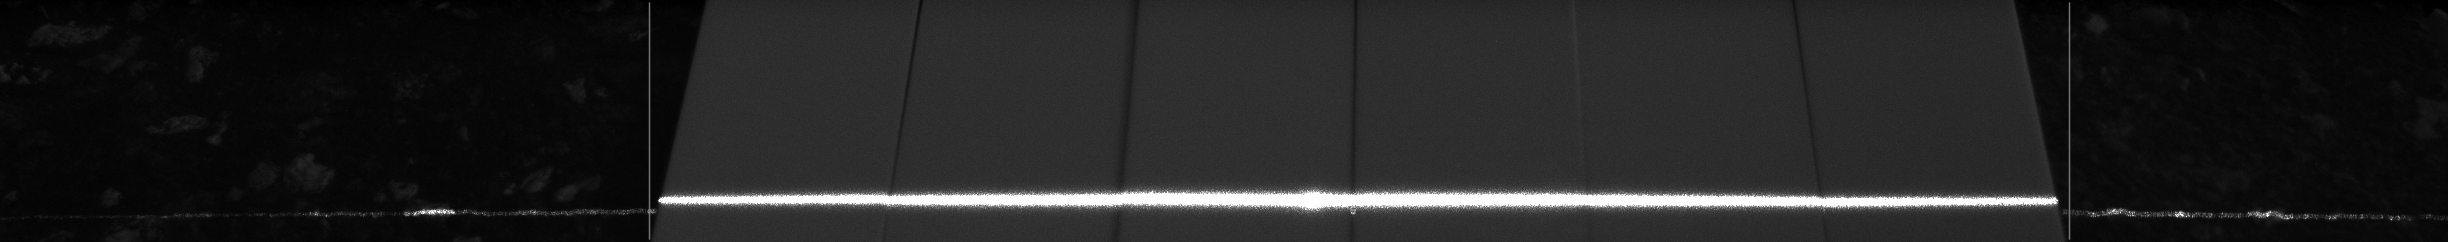
\includegraphics[width=0.8\linewidth]{Billeder/_1_normal}
	\caption{Stribens lokation}
	\label{fig:1normal}
\end{figure}

Ud fra lokationerne af de to sider, dannes et område der afgrænser kanterne af striben. Området benyttes til at danne afgrænsninger af de tre hovedområder, hvor striben er og hvor den ikke er.

\newpage

\subsection{Laseren uden for striben}

Ved brug af det afgrænsede område fra sektion \ref{ref::stribefind}, antages det at laseren vil befinde sig i den nederste kvarte del af billedet. Hvis det ikke er tilfældet, er lokationen af måleenheden i forhold til striben ikke egnet til at måle fra.
\begin{figure}[h]
	\centering
	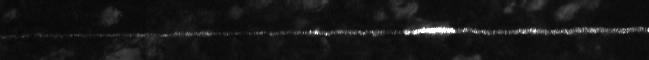
\includegraphics[width=0.7\linewidth]{Billeder/base_1_filter}
	\caption{Laseren uden for striben, filtreret}
	\label{fig:base_1_filter}
\end{figure}

Når afgrænsningen er foretaget, bliver området filtreret med et filter der hjælper med at lokalisere laseren via en hertil valgt kernel. Her illustreret af figur \ref{fig:base_1_filter}.

\begin{figure}[h]
	\centering
	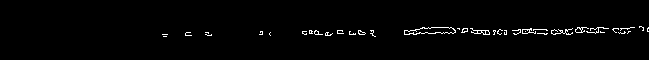
\includegraphics[width=0.7\linewidth]{Billeder/base_2_canny}
	\caption{Lasere efter edge detection}
	\label{fig:base_2_canny}
\end{figure}

Herefter bliver dataen manipuleret i samme stil som i sektion \ref{ref::stribefind}.

Grundet det faktum at laserens repræsentation ved siden af striben ikke er så tydelig, bliver billedet herefter behandlet via en gradient morphology algoritme, der sørger for at lukke små huller ud fra Canny algoritmens resultat.

\begin{figure}[h]
	\centering
	
\includegraphics[width=0.7\linewidth]{Billeder/base_3_morph}
	\caption{Lasere efter gradient morphology}
	\label{fig:base_3_morph}
\end{figure}

På dette punkt er informationerne tilstrækkelig rige til at kunne benytte en properlistisk houghlines algoritme til at lokalisere det område hvor laseren befinder sig.

\begin{figure}[h!]
	\centering
	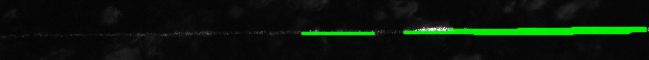
\includegraphics[width=0.7\linewidth]{Billeder/base_4_houghP}
	\caption{Houghlines finder linjer}
	\label{fig:base_4_hough}
\end{figure}

Ud fra de informationer der bliver dannet via houghlines, kan laseren komplette område rammes ind. Herefter følger en vægtning af det indrammede information der er beskrevet mere detaljeret i sektion \ref{ref::weight}.

\subsection{Laseren på striben}
Informationerne i den del af billedet er temmelig anderledes, grundet laserens placering oven på vejstriben. Derfor kan der tages udgangspunkt i den originale eksponering da denne var den lavest mulige til at kunne identificere vejstriben. Det resulterer i at selve laseren vil have en meget høj intensitet i forhold til resten, og det udnyttes til at kunne adskille den position hvor den er ret nemt. Laserens billede bliver udglattet for at modvirke eventuelle mindre overlapninger fra laser til stribe i intensitet hvor det ikke ville være muligt at identificere hvad der hører til laseren og hvad der hører til striben. Når antagelsen af hvor laserens lokation er fundet, bliver dennes data også positionsvægtet, hvilket er beskrevet i sektion \ref{ref::weight}.

\subsection{Vægtet placering\label{ref::weight}}
Algoritmen benytter sig af moments, og mere specifikt \texttt{m01} og \texttt{m00} til at udregne vægtningerne.
Den opbygger en liste af punkter, hvor alle X-koordinaterne befinder sig i stigende orden fra 0 til N, hvor N i dette tilfælde er bredden af det billede den skal bearbejde.
Y-koordinaterne bliver sat ud fra det billede der skal bearbejdes. Den vil opdele billedet i små bidder der er præcis 1 pixel bred, og derefter udfører moments algoritmen på hver af disse bidder. Det resulterer i en enkelt værdi, der er det vægtede punkt i Y, for lige præcis den X. Denne Y-værdi bliver indsat i punktlisten og derved indeholder listen en komplet vægtning i Y for pixel intensiteter, for alle X i et givent billede. Meta data, der omhandler den reale lokation for den udregnede punktliste, bør opbevares andet steds.

\begin{figure}[h]
	\centering
	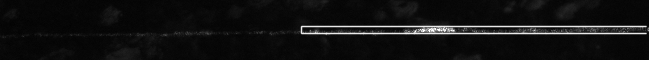
\includegraphics[width=0.7\linewidth]{Billeder/base_5_boxing}
	\caption{Det område der skal udføres intensitetsbaseret vægtning af laseren}
	\label{fig:base_5_boxing}
\end{figure}

\subsection{Højden}
Alt ud fra hvorledes højden ønskes beregnet, f.eks. gennemsnit af de fundne lokationer, kan de gemte data udregnes på den ønskede måde. Dataen i dens rå form åbner op for, at på forskellig vis kunne behandle dem, og opnå de informationer man ønsker.


	
	\section{Fejlede forsøg}
Undervejs i forløbet er forskellige metoder til stadierne i processen blevet afprøvet, hvoraf alle endte med at blive skrottet. Sektionen beskriver de forskellige procedurer, hvilket problem de skulle løse og hvad ideen bag dem var, og hvorfor de ikke var brugbare i praksis.

\subsection{Diagonal matricer}

\subsubsection{Problemstilling}
Identificering af start og slutpunkter for laseren på striben

\subsubsection{Metode}
Metoden er, at opdele billedet i diagonale matricer for derefter at gennemløbe disse for at identificere dobbeltskæringer af laseren. Selve billedet ville blive opdelt i matricer,  i samme antal, som det dobbelte af billedets højde, på begge leder. Det ville resultere i et net af matricer på tværs i begge retninger, hvor pixel intensitetsforskelle for hver i forhold til dens naboer ville medføre et slags toppunkt. I tilfælde af at to var tilstede og de matchede med naboerne, kunne denne information benyttes til at søge efter intensitets variationer, der i sidste ende ville medføre at en potentiel lokation, der kunne bruges, var fundet.

\subsubsection{Resultat}
Metoden viste sig at være utroligt krævende, både med hensyn til design og regnekraft samt noget utilregnelig. Under perfekte situationer virkede det nogenlunde, og hvis der var nogen diskrepans i laserens position grundet støj eller andre elementer ville den give resultater der ikke kunne bruges. Den blev derfor kasseret i et forholdsvis tidligt stadie da det ikke var rentabelt at gå videre i denne retning.

\subsection{Differentiering}

\subsubsection{Problemstilling}
Lokalisering af laser på stribe kontra jord.

\subsubsection{Metode}
Ved at tage alle punkter i X-aksen, og tage forskellen på dem i stigende orden, ville det være muligt at se om et givent koordinat steg eller faldt i højde.
Denne process udføres to gange, for at få absolutte værdier der indikerer udsving i niveau. Ved at finde de største af disse var forhåbningen af det kunne bruges til at finde ud af hvor den stigning laseren var på striben befandt sig.

\subsubsection{Resultat}
I teorien var det en fantastisk ide, men det forblev også kun i teorien. I praksis viste metoden sig at være ubrugelig, fordi afveksling af laserens intensitet på jorden, f.eks. fra fremmedlegemer såsom småsten eller deres refleksioner herfra gjorde det umuligt, at være sikker på om de punkter, der blev lokaliseret rent faktisk var stribens position, eller noget der var en afvigelse fra et helt andet sted.
På trods af det, var det en ganske effektiv og simpel metode til at identificere niveauvariationer.

\subsection{Histogram}

\subsubsection{Problemstilling}
Lokalisering af stribe

\subsubsection{Metode}
Ved at opdele alle billedets pixels i et intensitets histogram kunne de forskellige intensiteter være med til at identificere hvilke der tilhørte striben og derved lokalisere dens position.

\subsubsection{Nødvendigheder}
Algoritmer til at identificere højde- og lavpunkter ud fra data samt en manuel opbygget histogram datastruktur.

\subsubsection{Resultat}
I teorien skulle metoden være mulig, men her opstod et problem der ikke var forudset. Intensiteten af pixels for
\begin{itemize}
	\item Stribe med og uden laser
	\item Jord med og uden laser
\end{itemize}
befandt sig inden for et så lille område at det praktisk var umuligt at foretage udvælgelse af værdierne for videre identificering. Det fremgik også at der, på trods af udelukkelse af for mørke dele, ikke var mulighed for at garantere hvilke intensiteter der tilhørte hvad. Dette forsagede desværre også at det ikke var muligt at søge efter intensitetsgrænser.
Derudover blev situationen heller ikke forbedret af eksponerings problematikker og støv på kamerachippen osv.
Det havde den effekt at det var stort set umuligt at separere de forskellige elementer da overgangene var utroligt ustabile og kunne blive influeret af hvad som helst. På den lyse side blev der dog udviklet to algoritmer, en til at finde højdepunkter og en til at finde lavpunkter, der begge er justerbare med forskellige parametre.
\newpage
\subsection{Nærheds højdemåling}
\subsubsection{Problemstilling}
Undgå indflydelse fra skæv laser ved måling af højden.

\subsubsection{Metode}
Grundet laserens bueform, blev to små bider af laseren udskåret. Hvis disse faldt inde for samme vinkel ville betydningen af laserens bueform have minimal indflydelse. Desværre er denne metode ikke præcis nok da den ikke tager højde for bl.a. udsving i laserens intensitetsvariationer over tid eller elementer der kunne være betydningsfulde for målingen som f.eks. fremmedlegemer.

\subsubsection{Resultat}
Målinger foretaget ved denne metode viser markant andre værdier, og er temmelig svingene i resultater.

	
	
	\bibliographystyle{unsrt}
	\bibliography{ref}
	
\end{document}
